\hypertarget{section-building-block-view}{%
\section{5 Building Block View}\label{section-building-block-view}}

\textbf{Content}

The building block view shows the static decomposition of the system into building blocks (modules, components, subsystems, classes, interfaces, packages, libraries, frameworks, layers, partitions, tiers, functions, operations, \ldots) or their relationships and associations. It helps to maintain an overview of your source code by making its structure understandable through abstraction.

\subsection{Component-Based Frontend Architecture}
The Vivendo webshop frontend follows a \textbf{component-based modular frontend design}. The different modules are interconnected to provide a seamless shopping experience. The primary technologies used include \textbf{Next.js, Tailwind CSS}, API integration and Context API for state management. This approach ensures:
\begin{itemize}
    \item Clear separation of concerns through distinct modules.
    \item Reusability of components across different sections.
    \item Better maintainability and scalability.
    \item Efficient state and API management.
\end{itemize}
The architectural overview is depicted in the figure below:

\begin{figure}[h]
    \centering
    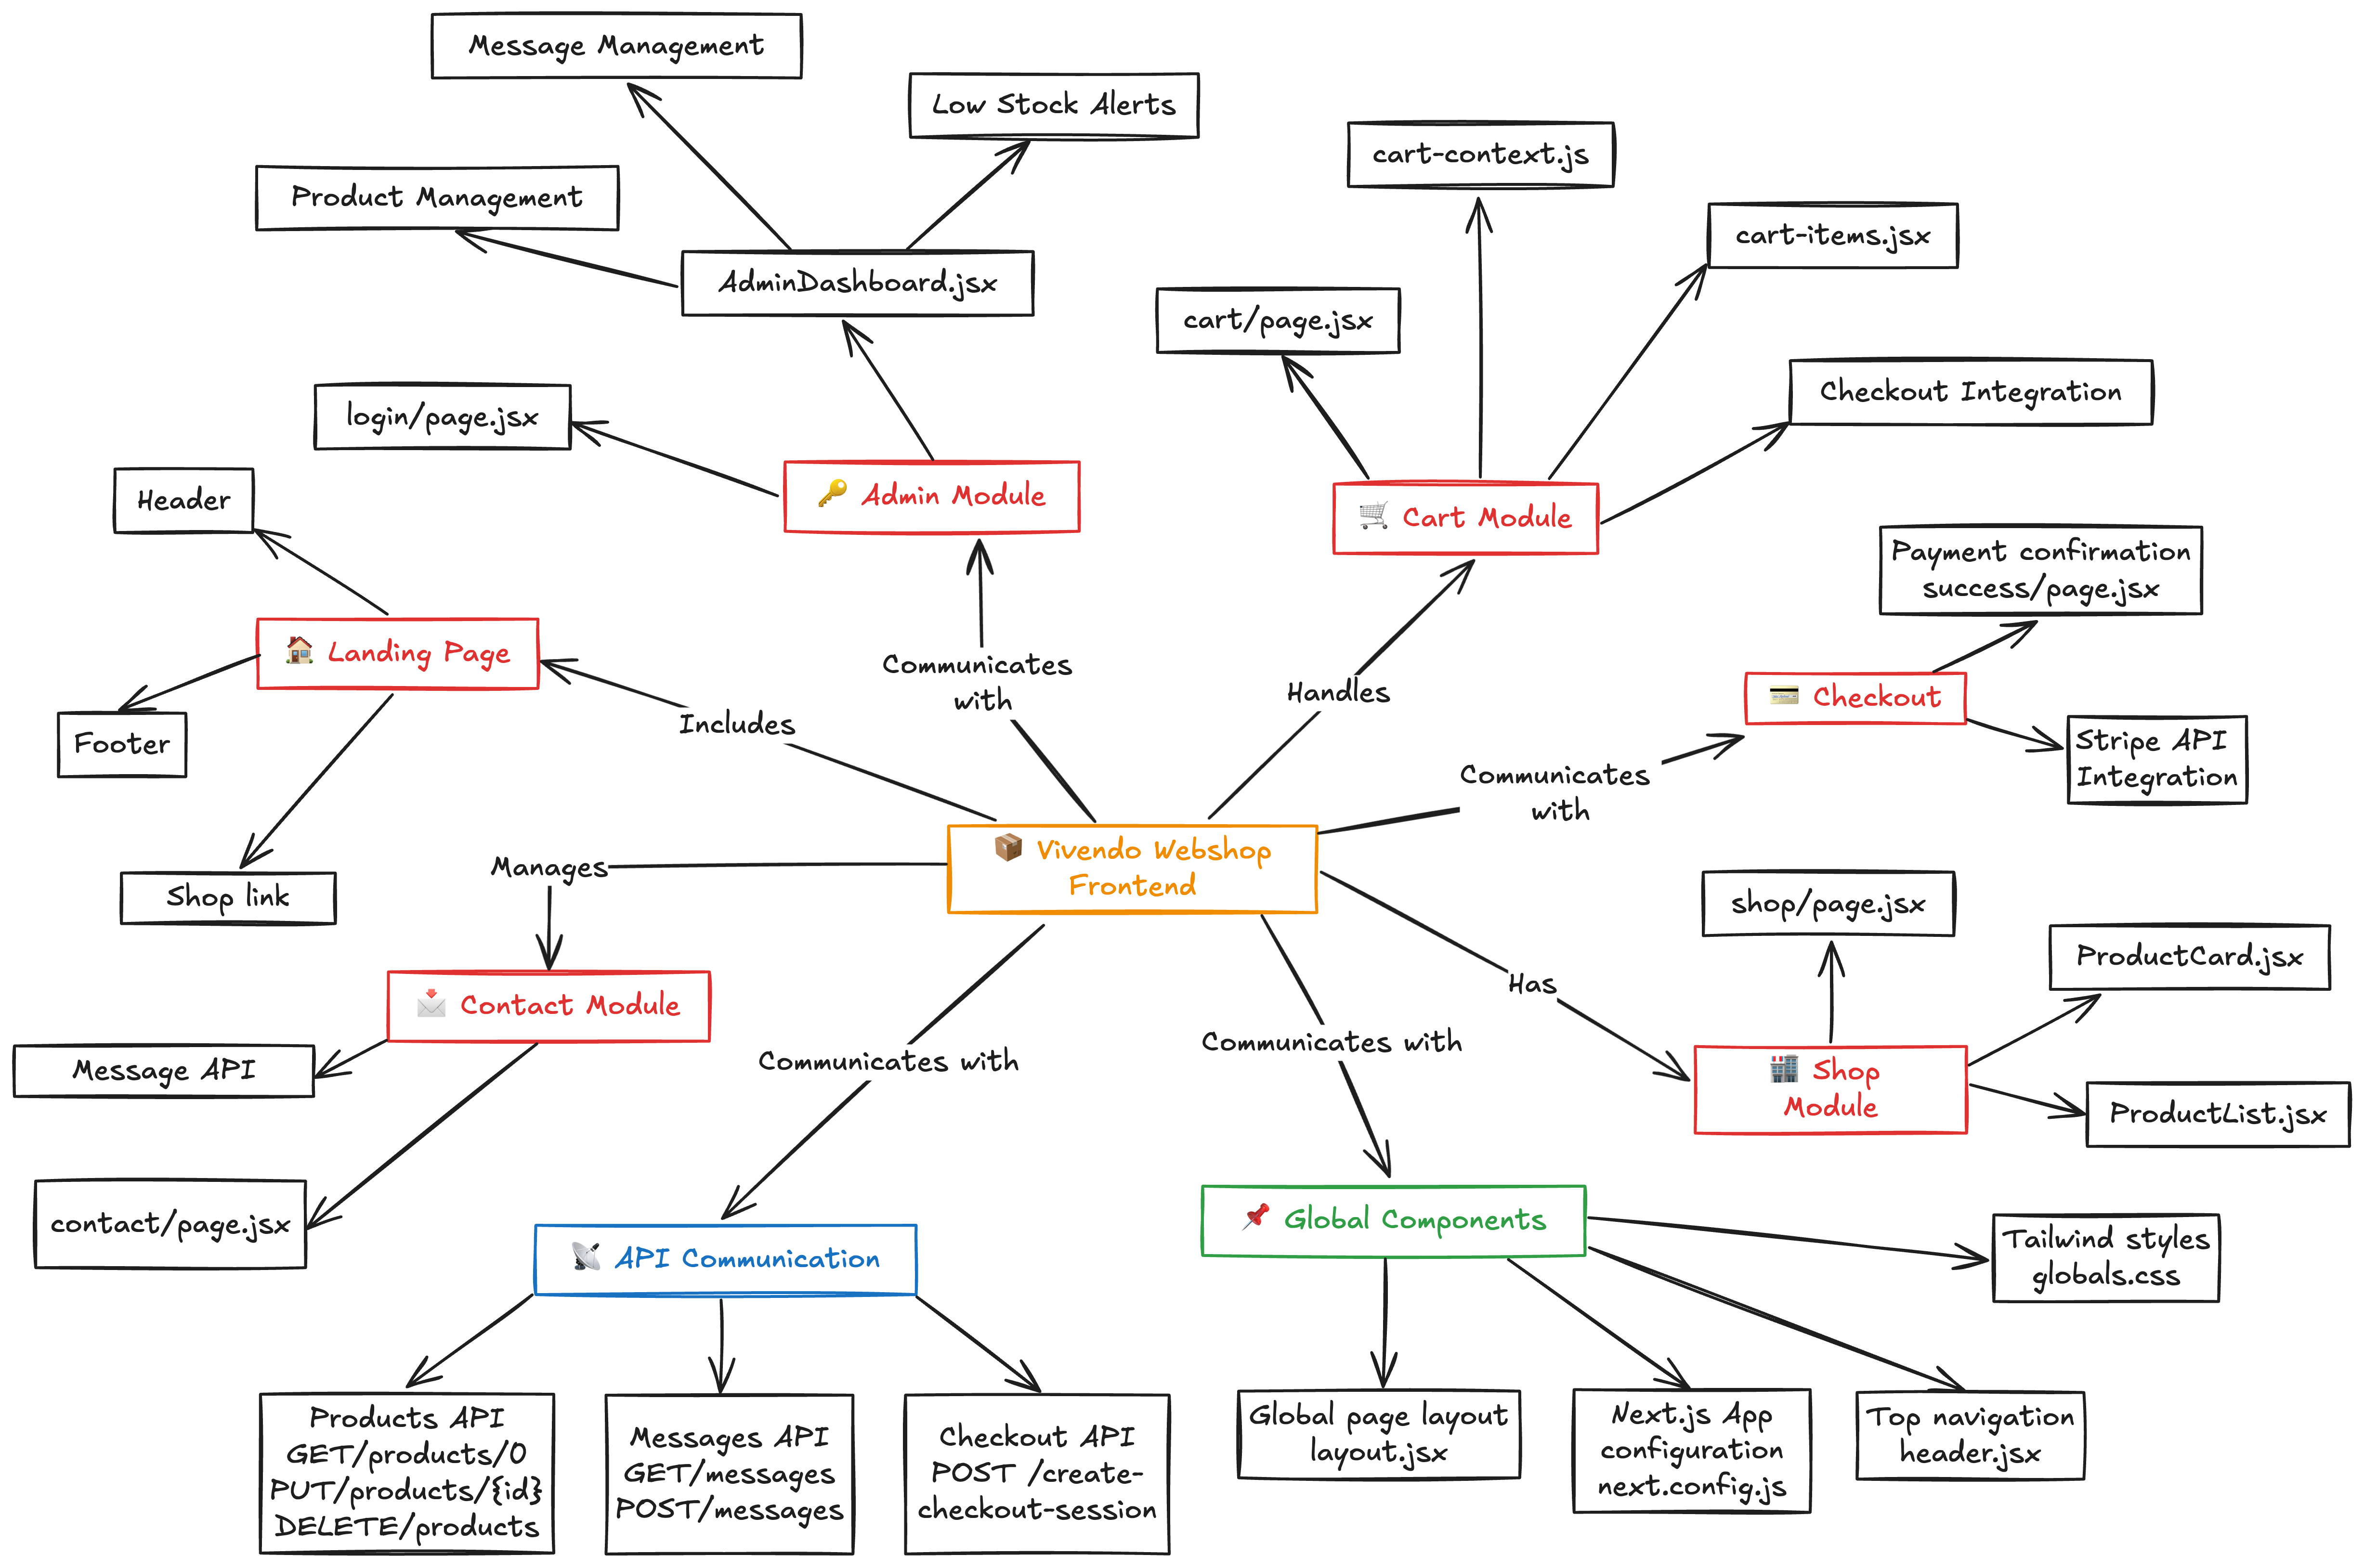
\includegraphics[width=\textwidth]{images/New_frontend_architecture.png}
    \caption{Component-Based Frontend Architecture}
    \label{fig:architecture}
\end{figure}

\subsection{Core Frontend Modules and Interactions}
The system consists of several modules:
\begin{itemize}
    \item \textbf{Landing Page Module}: Includes key UI components such as the header, footer and navigation links.
    \item \textbf{Admin Module}: Manages the admin dashboard, including product management, low stock alerts and message management. The admin module is responsible for managing products, messages, and stock alerts. It is connected to the \textbf{Admin Dashboard} component, which communicates with the API layer.
    \item \textbf{Cart Module}: Handles cart functionality, including cart context, cart items and checkout integration. The cart module manages cart-related functionalities and state using \texttt{cart-context.js}. It also connects with the checkout module to handle Stripe payments.
    \item \textbf{Shop Module}: Displays product listings and product cards with interactivity.
    \item \textbf{Checkout Module}: Integrates with Stripe API for handling payments and success confirmations.
    \item \textbf{Contact Module}: Manages user interactions via the contact page and handles message submissions. It connects with the API layer to store and retrieve messages.
    \item \textbf{API Communication Layer}: Manages requests to the backend services, including product APIs, messages API and checkout API. This layer serves as the middleware between the frontend and backend, making requests via REST APIs. It handles product data, message submissions, and checkout sessions.
    \item \textbf{Global Components}: Includes shared layout elements, styles and configurations.
\end{itemize}

%% 

%% ADD BACKEND BUILDING BLOCK VIEW PART / ARCHITECTURE HERE

%% TEMPLATE CONTENT BELOW HERE %%

\textbf{Form}

The building block view is a hierarchical collection of black boxes and
white boxes (see figure below) and their descriptions.

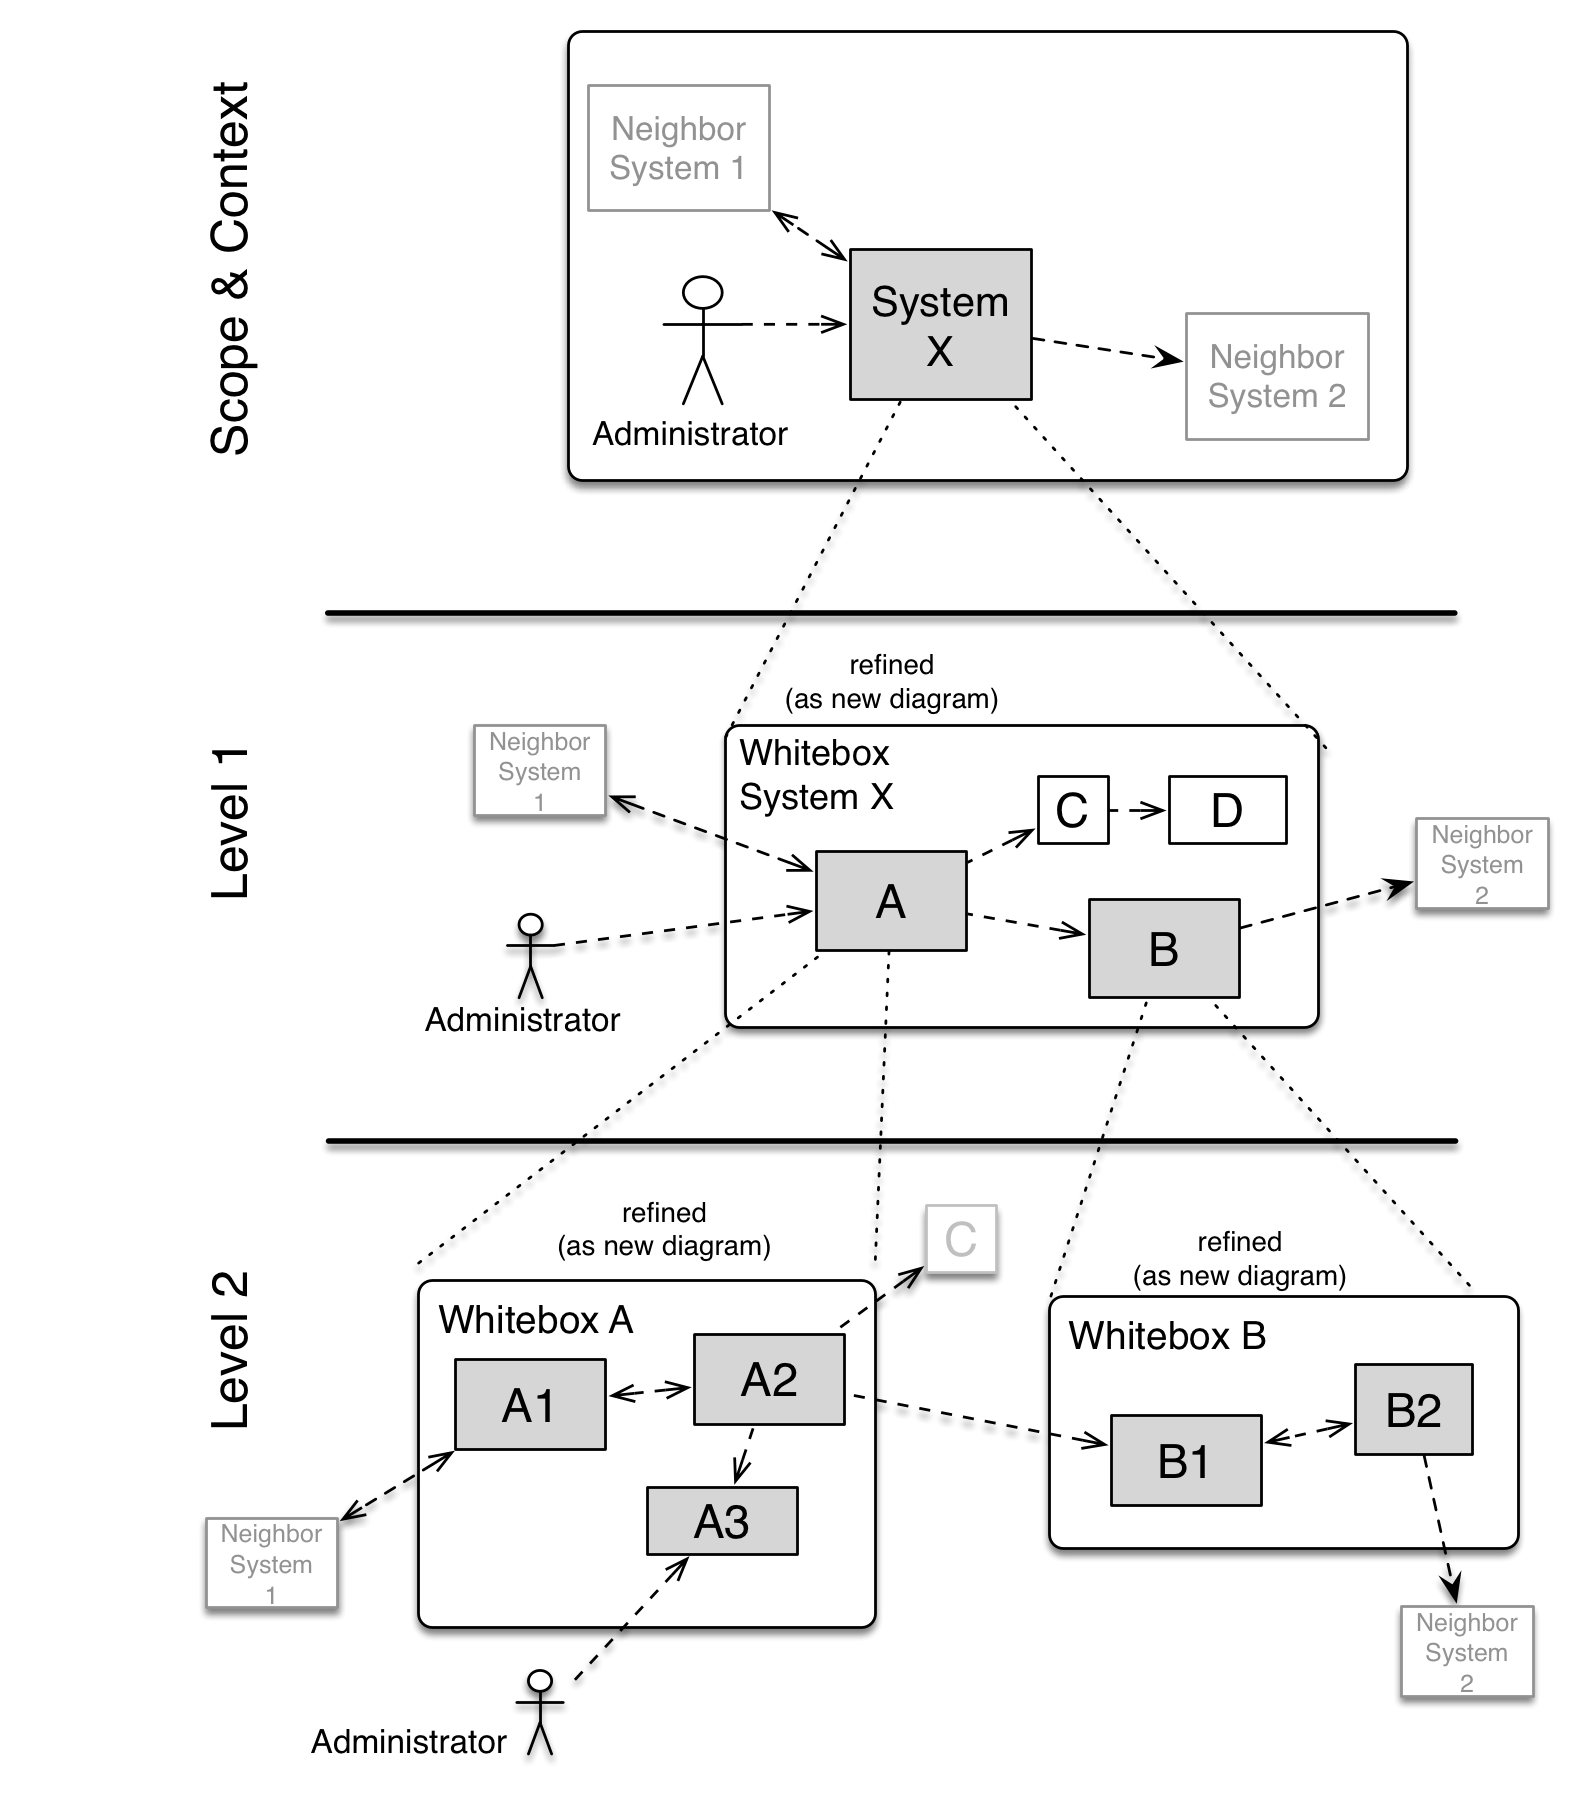
\includegraphics{images/05_building_blocks-EN.png}

\textbf{Level 1} is the white box description of the overall system
together with black box descriptions of all contained building blocks.

\textbf{Level 2} zooms into some building blocks of level 1. Thus it
contains the white box description of selected building blocks of level
1, together with black box descriptions of their internal building
blocks.

\textbf{Level 3} zooms into selected building blocks of level 2, and so
on.

See \href{https://docs.arc42.org/section-5/}{Building Block View} in the
arc42 documentation.

\hypertarget{_whitebox_overall_system}{%
\subsection{Whitebox Overall System}\label{_whitebox_overall_system}}

Here you describe the decomposition of the overall system using the
following white box template. It contains

\begin{itemize}
\item
  an overview diagram
\item
  a motivation for the decomposition
\item
  black box descriptions of the contained building blocks. For these we
  offer you alternatives:

  \begin{itemize}
  \item
    use \emph{one} table for a short and pragmatic overview of all
    contained building blocks and their interfaces
  \item
    use a list of black box descriptions of the building blocks
    according to the black box template (see below). Depending on your
    choice of tool this list could be sub-chapters (in text files),
    sub-pages (in a Wiki) or nested elements (in a modeling tool).
  \end{itemize}
\item
  (optional:) important interfaces, that are not explained in the black
  box templates of a building block, but are very important for
  understanding the white box. Since there are so many ways to specify
  interfaces why do not provide a specific template for them. In the
  worst case you have to specify and describe syntax, semantics,
  protocols, error handling, restrictions, versions, qualities,
  necessary compatibilities and many things more. In the best case you
  will get away with examples or simple signatures.
\end{itemize}

\emph{\textbf{\textless Overview Diagram\textgreater{}}}

\begin{description}
\item[Motivation]
\emph{\textless text explanation\textgreater{}}
\item[Contained Building Blocks]
\emph{\textless Description of contained building block (black
boxes)\textgreater{}}
\item[Important Interfaces]
\emph{\textless Description of important interfaces\textgreater{}}
\end{description}

Insert your explanations of black boxes from level 1:

If you use tabular form you will only describe your black boxes with
name and responsibility according to the following schema:

\begin{longtable}[]{@{}
  >{\raggedright\arraybackslash}p{(\columnwidth - 2\tabcolsep) * \real{0.3333}}
  >{\raggedright\arraybackslash}p{(\columnwidth - 2\tabcolsep) * \real{0.6667}}@{}}
\toprule
\begin{minipage}[b]{\linewidth}\raggedright
\textbf{Name}
\end{minipage} & \begin{minipage}[b]{\linewidth}\raggedright
\textbf{Responsibility}
\end{minipage} \\
\midrule
\endhead
\emph{\textless black box 1\textgreater{}} &
~\emph{\textless Text\textgreater{}} \\
\emph{\textless black box 2\textgreater{}} &
~\emph{\textless Text\textgreater{}} \\
\bottomrule
\end{longtable}

If you use a list of black box descriptions then you fill in a separate
black box template for every important building block . Its headline is
the name of the black box.

\hypertarget{__name_black_box_1}{%
\subsubsection{\textless Name black box
1\textgreater{}}\label{__name_black_box_1}}

Here you describe \textless black box 1\textgreater{} according the the
following black box template:

\begin{itemize}
\item
  Purpose/Responsibility
\item
  Interface(s), when they are not extracted as separate paragraphs. This
  interfaces may include qualities and performance characteristics.
\item
  (Optional) Quality-/Performance characteristics of the black box,
  e.g.availability, run time behavior, \ldots.
\item
  (Optional) directory/file location
\item
  (Optional) Fulfilled requirements (if you need traceability to
  requirements).
\item
  (Optional) Open issues/problems/risks
\end{itemize}

\emph{\textless Purpose/Responsibility\textgreater{}}

\emph{\textless Interface(s)\textgreater{}}

\emph{\textless(Optional) Quality/Performance
Characteristics\textgreater{}}

\emph{\textless(Optional) Directory/File Location\textgreater{}}

\emph{\textless(Optional) Fulfilled Requirements\textgreater{}}

\emph{\textless(optional) Open Issues/Problems/Risks\textgreater{}}

\hypertarget{__name_black_box_2}{%
\subsubsection{\textless Name black box
2\textgreater{}}\label{__name_black_box_2}}

\emph{\textless black box template\textgreater{}}

\hypertarget{__name_black_box_n}{%
\subsubsection{\textless Name black box
n\textgreater{}}\label{__name_black_box_n}}

\emph{\textless black box template\textgreater{}}

\hypertarget{__name_interface_1}{%
\subsubsection{\textless Name interface
1\textgreater{}}\label{__name_interface_1}}

\ldots{}

\hypertarget{__name_interface_m}{%
\subsubsection{\textless Name interface
m\textgreater{}}\label{__name_interface_m}}

\hypertarget{_level_2}{%
\subsection{Level 2}\label{_level_2}}

Here you can specify the inner structure of (some) building blocks from
level 1 as white boxes.

You have to decide which building blocks of your system are important
enough to justify such a detailed description. Please prefer relevance
over completeness. Specify important, surprising, risky, complex or
volatile building blocks. Leave out normal, simple, boring or
standardized parts of your system

\hypertarget{_white_box_emphasis_building_block_1_emphasis}{%
\subsubsection{\texorpdfstring{White Box \emph{\textless building block
1\textgreater{}}}{White Box \textless building block 1\textgreater{}}}\label{_white_box_emphasis_building_block_1_emphasis}}

\ldots describes the internal structure of \emph{building block 1}.

\emph{\textless white box template\textgreater{}}

\hypertarget{_white_box_emphasis_building_block_2_emphasis}{%
\subsubsection{\texorpdfstring{White Box \emph{\textless building block
2\textgreater{}}}{White Box \textless building block 2\textgreater{}}}\label{_white_box_emphasis_building_block_2_emphasis}}

\emph{\textless white box template\textgreater{}}

\ldots{}

\hypertarget{_white_box_emphasis_building_block_m_emphasis}{%
\subsubsection{\texorpdfstring{White Box \emph{\textless building block
m\textgreater{}}}{White Box \textless building block m\textgreater{}}}\label{_white_box_emphasis_building_block_m_emphasis}}

\emph{\textless white box template\textgreater{}}

\hypertarget{_level_3}{%
\subsection{Level 3}\label{_level_3}}

Here you can specify the inner structure of (some) building blocks from
level 2 as white boxes.

When you need more detailed levels of your architecture please copy this
part of arc42 for additional levels.

\hypertarget{_white_box_building_block_x_1}{%
\subsubsection{White Box \textless\_building block
x.1\_\textgreater{}}\label{_white_box_building_block_x_1}}

Specifies the internal structure of \emph{building block x.1}.

\emph{\textless white box template\textgreater{}}

\hypertarget{_white_box_building_block_x_2}{%
\subsubsection{White Box \textless\_building block
x.2\_\textgreater{}}\label{_white_box_building_block_x_2}}

\emph{\textless white box template\textgreater{}}

\hypertarget{_white_box_building_block_y_1}{%
\subsubsection{White Box \textless\_building block
y.1\_\textgreater{}}\label{_white_box_building_block_y_1}}

\emph{\textless white box template\textgreater{}}
